\section{Indices: the ultimate rizzler!}
Indices make our lives easier when writing abstract quantitites having multiple components, like vectors. If we have a three-dimensional vector, we can write it as $v\indices{^i}$ where $i$ can take the values $1$, $2$, or $3$.\\[0.3cm]
 Why are the indices written as superscript? Well, these are contravariant indices which will be discussed later. For now, let just say that `upstairs' indices are the `normal thing'. Index placement is important and these are not powers...just the way we denote the components.\\[0.3cm]
 Consider the (in)famous equation: 
 $$\mathbf{F}= m \mathbf{a}$$
 This can be written as $F\indices{^i} = m a\indices{^i}$, for each component $i$. Just remember that we should have the same kind of indices on both side of the equation finally. That is, if we have `upstairs' index on the right, same should be on the left.\\[0.3cm]
 \subsection{Einstein Convention}
 The OG rule...whenever you see two same indices, sum them.  That's it! Let's make our hands dirty and look at some examples:\\[0.3cm]
 \subsection{Examples}
 \textbf{Matrix Multiplication:}\\[0.3cm]
 Let us have the eigenvalue equation $M\mathbf{v} = \lambda\mathbf{v}$. We can write this as: 
 $$\sum\limits_j M_{ij}v^j = \lambda v^i$$
 Note two things here: 
 \begin{itemize}
    \item The index $j$ is summed over, so it does not come in the final expression (dummy index!).
    \item The index $i$ occurs as a superscript on the right, so in the left also, the final expression should have the index $i$ as a superscript.
 \end{itemize}
 Thus, using Einstein convention and correct index placement, the above equation can be written as:
$$M\indices*{^i_j}v\indices{^j} = \lambda v\indices{^i}$$
This can be visualised by treating each quantity as a `box' with the indices as some `hands' portruding out. When we sum, we just join these `hands'. After taking the sum, the number of free hands decreases (index contraction)l A matrix has two hands and a vector has one hand. When we multiply a matrix with a vector, we obtain a vector, which should have one hand. This is represented in the diagram below:
\begin{figure}[H]
    \centering
    

\tikzset{every picture/.style={line width=0.75pt}} %set default line width to 0.75pt        

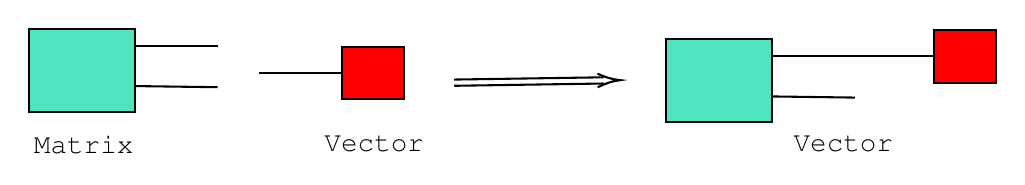
\begin{tikzpicture}[x=0.75pt,y=0.75pt,yscale=-1,xscale=1]
%uncomment if require: \path (0,300); %set diagram left start at 0, and has height of 300

%Shape: Rectangle [id:dp9056942194735556] 
\draw  [fill={rgb, 255:red, 80; green, 227; blue, 194 }  ,fill opacity=1 ] (100,112) -- (151,112) -- (151,152) -- (100,152) -- cycle ;
%Straight Lines [id:da9172659624339214] 
\draw [fill={rgb, 255:red, 80; green, 227; blue, 194 }  ,fill opacity=1 ]   (151,120.18) -- (191,120.18) ;
%Straight Lines [id:da2833939201314972] 
\draw [fill={rgb, 255:red, 80; green, 227; blue, 194 }  ,fill opacity=1 ]   (151,139.63) -- (191,140.18) ;

%Shape: Rectangle [id:dp6422275710126122] 
\draw  [fill={rgb, 255:red, 255; green, 0; blue, 0 }  ,fill opacity=1 ] (251,120.63) -- (281,120.63) -- (281,146) -- (251,146) -- cycle ;
%Straight Lines [id:da9091154996581836] 
\draw [fill={rgb, 255:red, 255; green, 0; blue, 0 }  ,fill opacity=1 ]   (211,133.18) -- (251,133.18) ;

%Straight Lines [id:da6668729559343063] 
\draw    (304.98,136.5) -- (376.98,135.41)(305.02,139.5) -- (377.02,138.4) ;
\draw [shift={(385,136.78)}, rotate = 179.13] [color={rgb, 255:red, 0; green, 0; blue, 0 }  ][line width=0.75]    (10.93,-3.29) .. controls (6.95,-1.4) and (3.31,-0.3) .. (0,0) .. controls (3.31,0.3) and (6.95,1.4) .. (10.93,3.29)   ;
%Shape: Rectangle [id:dp5499160435625281] 
\draw  [fill={rgb, 255:red, 80; green, 227; blue, 194 }  ,fill opacity=1 ] (407,117) -- (458,117) -- (458,157) -- (407,157) -- cycle ;
%Straight Lines [id:da11942666503370314] 
\draw [fill={rgb, 255:red, 80; green, 227; blue, 194 }  ,fill opacity=1 ]   (458,125.18) -- (498,125.18) ;
%Straight Lines [id:da4684372747610551] 
\draw [fill={rgb, 255:red, 80; green, 227; blue, 194 }  ,fill opacity=1 ]   (458,144.63) -- (498,145.18) ;

%Shape: Rectangle [id:dp9126568397813256] 
\draw  [fill={rgb, 255:red, 255; green, 0; blue, 0 }  ,fill opacity=1 ] (536,112.63) -- (566,112.63) -- (566,138) -- (536,138) -- cycle ;
%Straight Lines [id:da5617556659509985] 
\draw [fill={rgb, 255:red, 255; green, 0; blue, 0 }  ,fill opacity=1 ]   (496,125.18) -- (536,125.18) ;


% Text Node
\draw (101,162) node [anchor=north west][inner sep=0.75pt]   [align=left] {{\fontfamily{pcr}\selectfont Matrix}};
% Text Node
\draw (241,162) node [anchor=north west][inner sep=0.75pt]   [align=left] {{\fontfamily{pcr}\selectfont Vector}};
% Text Node
\draw (467,162) node [anchor=north west][inner sep=0.75pt]   [align=left] {{\fontfamily{pcr}\selectfont Vector}};


\end{tikzpicture}

    \caption{Matrix-vector multiplication. The final product has one free hand and is thus a vector.}
\end{figure}
\noindent
\textbf{The Scalar Product:}\\[0.3cm]
The dot product or scalar product of two vectors is a scalar (no hand). Then, there should be no free index in the expression. Thus, in the index notation:
$$\mathbf{v}\cdot \mathbf{v} = v\indices{^i}v\indices{_i} =v\indices{_i}v\indices{^i}  $$
The last two expressions are same. The upstairs or downstairs indices do not matter, as these are summed over. Note that in this definition, we have used a \textit{dual vector}, having a lower index. We can also define the dot product using the \textit{regular} vector with an upper index but then a \textit{metric} comes in.
\begin{figure}[H]
    \centering
    

\tikzset{every picture/.style={line width=0.75pt}} %set default line width to 0.75pt        

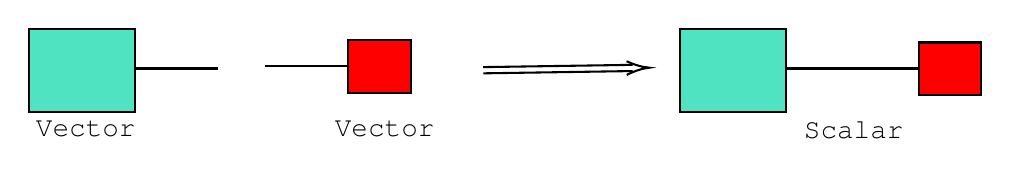
\begin{tikzpicture}[x=0.75pt,y=0.75pt,yscale=-1,xscale=1]
%uncomment if require: \path (0,300); %set diagram left start at 0, and has height of 300

%Shape: Rectangle [id:dp5798300081474196] 
\draw  [fill={rgb, 255:red, 80; green, 227; blue, 194 }  ,fill opacity=1 ] (100,112) -- (151,112) -- (151,152) -- (100,152) -- cycle ;
%Straight Lines [id:da22962560201461135] 
\draw [fill={rgb, 255:red, 80; green, 227; blue, 194 }  ,fill opacity=1 ]   (151,131.18) -- (191,131.18) ;
%Shape: Rectangle [id:dp20432070859726514] 
\draw  [fill={rgb, 255:red, 255; green, 0; blue, 0 }  ,fill opacity=1 ] (254,117.63) -- (284,117.63) -- (284,143) -- (254,143) -- cycle ;
%Straight Lines [id:da524122200138993] 
\draw [fill={rgb, 255:red, 255; green, 0; blue, 0 }  ,fill opacity=1 ]   (214,130.18) -- (254,130.18) ;

%Straight Lines [id:da7051909181445478] 
\draw    (318.98,130.5) -- (390.98,129.41)(319.02,133.5) -- (391.02,132.4) ;
\draw [shift={(399,130.78)}, rotate = 179.13] [color={rgb, 255:red, 0; green, 0; blue, 0 }  ][line width=0.75]    (10.93,-3.29) .. controls (6.95,-1.4) and (3.31,-0.3) .. (0,0) .. controls (3.31,0.3) and (6.95,1.4) .. (10.93,3.29)   ;
%Shape: Rectangle [id:dp6270655055347218] 
\draw  [fill={rgb, 255:red, 80; green, 227; blue, 194 }  ,fill opacity=1 ] (414,112) -- (465,112) -- (465,152) -- (414,152) -- cycle ;
%Straight Lines [id:da6216765005210074] 
\draw [fill={rgb, 255:red, 80; green, 227; blue, 194 }  ,fill opacity=1 ]   (465,131.18) -- (505,131.18) ;
%Shape: Rectangle [id:dp601921472040452] 
\draw  [fill={rgb, 255:red, 255; green, 0; blue, 0 }  ,fill opacity=1 ] (529,118.63) -- (559,118.63) -- (559,144) -- (529,144) -- cycle ;
%Straight Lines [id:da020089358658374357] 
\draw [fill={rgb, 255:red, 255; green, 0; blue, 0 }  ,fill opacity=1 ]   (489,131.18) -- (529,131.18) ;


% Text Node
\draw (102,155) node [anchor=north west][inner sep=0.75pt]   [align=left] {{\fontfamily{pcr}\selectfont Vector}};
% Text Node
\draw (246,155) node [anchor=north west][inner sep=0.75pt]   [align=left] {{\fontfamily{pcr}\selectfont Vector}};
% Text Node
\draw (472,155) node [anchor=north west][inner sep=0.75pt]   [align=left] {{\fontfamily{pcr}\selectfont Scalar}};


\end{tikzpicture}

    \caption{Dot product of two vectors. The final product is a scalar and has no free hands.}
\end{figure}
\noindent
So basically a \textit{scalar} is something that does not change under coordinate transformation, that is, if we go from a coordinate $(x,y,z)$ to $(x',y',z')$, a scale $\lambda = \lambda'$.\\[0.3cm]
\textbf{Euclidean Vectors:}\\[0.3cm]
Any vector can be written as in terms of basis vectors: $\mathbf{A} = \tensor{A}{^i}\mathbf{e}_i$ where $A^i$ are the components of the vector in the chosen basis. Now, we define $$\mathbf{e}_n\cdot \mathbf{e}_m = g_{nm}$$
These $g_{nm}$ are coefficients of metric tensor which will be discussed later. If these basis vectors are orthonormal, then the coefficients become the kronecker delta. Then we have the scalar product:
\begin{align*}
    \mathbf{A}\cdot \mathbf{B} &=  (\tensor{A}{^m}\mathbf{e}_m)\cdot  \tensor{B}{^n}\mathbf{e}_n\\
    &=(\tensor{A}{^m}\tensor{B}{^n}\mathbf{e}_m)\cdot  \mathbf{e}_n\\
    &=\tensor{A}{^m}\tensor{B}{^n}g_{nm}
\end{align*}
Note that we have used the \textit{regular vector} with an upper index here, with the metric $g$. We can define a cross product of two vectors as:
$$(\mathbf{A}\times \mathbf{B})^i = \epsilon^{ijk}A^jB^k$$
where $\epsilon^{ijk}$ is the Levi-Civita symbol (cyclic permutation of ${i,j,k}$ gives 1 and non-cyclic permutation gives -1 while repeated index in the symbol gives 0). \\[0.3cm]
\subsection{Some vector BS}
\textbf{Vectors as Directional Derivatives:}\\[0.3cm]
A vector can be thought of as a directional derivative. We define the directional derivative operator as:
$$\mathbf{v}\cdot \nabla = v^i \partial_i\equiv  v^i \dfrac{\partial}{\partial x^i}$$
This is very similar to the vector expansion in terms of the basis vectors. Thus, the partial derivatives somewhat act like a basis. The basis of partial derivatives is indeed called a \textit{coordinate basis}. Now let us calculate:
$$\mathbf{v}\cdot \nabla x^j = v^i \partial_i x^j = v^i\pdv{x^j}{x^i} = v^i\tensor*{\delta}{^j_i} = v^j$$
We have used the fact that coordinate components are independent of each other, that is, partial derivative of one component with respect to another gives a kronecker delta. Note that we have used the proper index placement here: $\partial_j\equiv \pdv{x^j}$ has a lower index (by definition) while $x^j$ has an upper index, thus kronecker delta has an upper as well as lower index.\\[0.3cm]
Now, let us consider we have a position vector written in a basis $\{\veb{e}_i\}$, that is, $$\veb{r} = x^i \veb{e}_i$$
Since $\veb{r}$ depends on the coordinate $\{x^i\}$, we can expand the differential displacement as:
\begin{align*}
    d\veb{r} &= \pdv{\veb{r}}{{x}^i}dx^i \\
    &= \pdv{(x^j \veb{e}_j)}{x^i}dx^i \\
    &=\brac{\pdv{x^j }{x^i}\veb{e}_j + \pdv{ \veb{e}_j}{x^i}x^j }dx^i
\end{align*}
The second term is zero as the basis vectors are independent of the coordinates and the first term gives Kronecker delta, thus we have:
$$d\veb{r} = \veb{e_i}dx^i $$
Comparing this with the first line of the previous expansion we have:
$$\boxed{\veb{e}_i = \pdv{\veb{r}}{x^i}}$$
Thus any basis vector can be obtained from the partial derivative of the position vector with respect to the coordinates.\\[0.3cm] 
\textbf{Vector Transformation:}\\[0.3cm]
Let us suppose we have a coordinate system $(x,y,z)$ and we rotate it about the $z$-axis by an angle $\theta$. The new coordinates are given by:
\begin{figure}[H]
    \centering 
    

\tikzset{every picture/.style={line width=0.75pt}} %set default line width to 0.75pt        

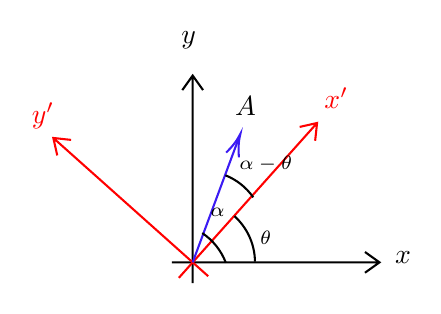
\begin{tikzpicture}[x=0.75pt,y=0.75pt,yscale=-1,xscale=1]
%uncomment if require: \path (0,201); %set diagram left start at 0, and has height of 201

%Shape: Axis 2D [id:dp5999262441064296] 
\draw  (283,150) -- (383,150)(293,60) -- (293,160) (376,145) -- (383,150) -- (376,155) (288,67) -- (293,60) -- (298,67)  ;
%Shape: Axis 2D [id:dp6999025250833045] 
\draw [color={rgb, 255:red, 255; green, 0; blue, 0 }  ,draw opacity=1 ] (286.34,157.46) -- (352.93,82.85)(225.85,90.07) -- (300.46,156.66) (344.54,84.75) -- (352.93,82.85) -- (352,91.41) (227.75,98.46) -- (225.85,90.07) -- (234.41,91)  ;
%Shape: Arc [id:dp9879953663640971] 
\draw  [draw opacity=0][line width=0.75]  (313.11,127.73) .. controls (319.05,133.11) and (322.85,140.84) .. (323,149.49) .. controls (323,149.54) and (323,149.6) .. (323,149.65) -- (293,150) -- cycle ; \draw  [line width=0.75]  (313.11,127.73) .. controls (319.05,133.11) and (322.85,140.84) .. (323,149.49) .. controls (323,149.54) and (323,149.6) .. (323,149.65) ;  
%Straight Lines [id:da08151702925178561] 
\draw [color={rgb, 255:red, 59; green, 27; blue, 243 }  ,draw opacity=1 ]   (293,150) -- (315.3,89.91) ;
\draw [shift={(316,88.03)}, rotate = 110.36] [color={rgb, 255:red, 59; green, 27; blue, 243 }  ,draw opacity=1 ][line width=0.75]    (10.93,-3.29) .. controls (6.95,-1.4) and (3.31,-0.3) .. (0,0) .. controls (3.31,0.3) and (6.95,1.4) .. (10.93,3.29)   ;
%Shape: Arc [id:dp7996887661941752] 
\draw  [draw opacity=0][line width=0.75]  (297.62,135.89) .. controls (302.69,139.3) and (306.73,144.24) .. (308.98,150.2) -- (280.91,160.81) -- cycle ; \draw  [line width=0.75]  (297.62,135.89) .. controls (302.69,139.3) and (306.73,144.24) .. (308.98,150.2) ;  
%Shape: Arc [id:dp8674168141053495] 
\draw  [draw opacity=0][line width=0.75]  (308.79,108.05) .. controls (314.04,110.15) and (318.74,113.75) .. (322.19,118.68) -- (297.62,135.89) -- cycle ; \draw  [line width=0.75]  (308.79,108.05) .. controls (314.04,110.15) and (318.74,113.75) .. (322.19,118.68) ;  

% Text Node
\draw (324,133.4) node [anchor=north west][inner sep=0.75pt]  [font=\scriptsize]  {$\theta $};
% Text Node
\draw (389,143.43) node [anchor=north west][inner sep=0.75pt]    {$x$};
% Text Node
\draw (286,37.43) node [anchor=north west][inner sep=0.75pt]    {$y$};
% Text Node
\draw (355,64.43) node [anchor=north west][inner sep=0.75pt]  [color={rgb, 255:red, 255; green, 0; blue, 0 }  ,opacity=1 ]  {$x'$};
% Text Node
\draw (214,71.43) node [anchor=north west][inner sep=0.75pt]  [color={rgb, 255:red, 255; green, 0; blue, 0 }  ,opacity=1 ]  {$y'$};
% Text Node
\draw (300,122.4) node [anchor=north west][inner sep=0.75pt]  [font=\scriptsize]  {$\alpha $};
% Text Node
\draw (312,68.43) node [anchor=north west][inner sep=0.75pt]    {$A$};
% Text Node
\draw (314,97.4) node [anchor=north west][inner sep=0.75pt]  [font=\scriptsize]  {$\alpha -\theta $};


\end{tikzpicture}
l
\end{figure}
$$x' = x\cos\theta - y\sin\theta$$
$$y' = x\sin\theta + y\cos\theta$$
$$z' = z$$
These relations can be readily found out using the following: Suppose we have a point $A$ making an angle $\alpha$ with the original system. Then we have $x = r\cos(\alpha), y = r\sin(\alpha)$. After rotation, the new coordinates are given by:
$$x' = r\cos(\alpha - \theta) = r\cos\alpha\cos\theta + r\sin\alpha\sin\theta$$
$$y' = r\sin(\alpha - \theta) = r\sin\alpha\cos\theta - r\cos\alpha\sin\theta$$
which gives the previous result. Note that the $z$ coordinate does not change as the rotation is about the $z$-axis. Now we consider the infinitesimal displacement in the new coordinate frame:
\begin{align*}
    (ds')^2 &= (dx')^2 + (dy')^2 + (dz')^2\\
    &= (dx\cos\theta - dy\sin\theta)^2 + (dx\sin\theta + dy\cos\theta)^2 + dz^2\\
    &= dx^2(\cos^2\theta+\sin^2\theta) + dy^2(\cos^2\theta+\sin^2\theta)- \cancel{2dxdy\sin\theta\cos\theta} +  \cancel{2dxdy\sin\theta\cos\theta} + dz^2\\
    &= dx^2 + dy^2 + dz^2\\
    &= ds^2
\end{align*}
Thus we see that the infinitesimal displacement is invariant under coordinate transformation and is thus a scalar.\\[0.3cm]
Now, note one thing: If we consider the new coordinates as a function of the old coordinate that is $x' \equiv x'(x,y,z)$, we can write: 
$$(dx')^i = \pdv{x'^i}{x^j}dx^j$$
Using this analogy, we can define the transformation of a vector as:
$$(v')^i = \pdv{x'^i}{x^j}v^j$$
Thus a vector is a quantity which transform like this. The terms $\pdv{x'^i}{x^j}$ are the components of the transformation matrix $\tensor*{\Lambda}{^i_j}$.
As we defined the transformation from $x$ to $x'$, we can also define the reverse transformation from $x'$ to $x$ as:
\begin{align*}
    x^i &= \pdv{x^i}{x'^j} x'^j \\
    & =  \brac{\pdv{x^i}{x'^j}\pdv{x'^j}{x^k}}x^k \\
\end{align*}
Now in the above sum, $j$ and $k$ indices are summed over. We must obtain $x^i$ from the right hand side also. Thus by observation, we can see that the term $\pdv{x^i}{x'^j}\pdv{x'^j}{x^k}$ must be equal to the kronecker delta $\tensor*{\delta}{^i_k}$.
